\documentclass[11pt,letterpaper]{article}

\usepackage[numbers,sort&compress]{natbib}
\usepackage{graphicx}
\usepackage{geometry}
\usepackage{amsmath}
\usepackage{amssymb}
\usepackage{booktabs}
\usepackage{xcolor}
\usepackage{listings}
\usepackage{url}
\usepackage{hyperref}

\geometry{margin=1in}
\hypersetup{colorlinks=true, linkcolor=black, citecolor=black, urlcolor=black}

\title{Decoy-Gated Neuro-Symbolic Extraction: A Label-Free FDR Gate at the Text-to-Logic Boundary and the Exchangeability Gap That Bounds It}

\author{Anonymous Authors\\ Affiliation Withheld for Review}
\date{}

\begin{document}

\maketitle

\begin{abstract}
Pipelines that translate short professional documents into executable first-order logic depend on an LLM to resolve fuzzy unifications, and that interface is exactly where plausible, high-confidence false facts enter and silently corrupt every downstream deduction. We import the knockoff / target-decoy machinery that genomics uses to control the false discovery rate (FDR) without labels, and build, to our knowledge, the first label-free FDR gate at this neural-to-symbolic admission boundary: before any LLM-proposed Prolog fact or bridge is admitted, it must out-score a plausibility-matched counterfactual decoy in a knockoff+ competition. We execute the protocol end to end and report measured outcomes, including those that disconfirm. Our central, surprising finding answers a prior methodology objection directly: re-run under the diagnostic-validated $K{=}5$ self-consistency elicitation, the gate fails to control FDR on the error-dense multi-hop family (realized FDR $1.0$ at the only certifiable target $\alpha^{*}{=}0.5$, bootstrap CI $[0.66,1.0]$)---even though the decoys are marginally exchangeable with the model's own spontaneous errors (KS $p{=}0.058$) and distinct from true positives (KS $p{=}5\times10^{-9}$). We localize the cause: marginal decoy exchangeability does not imply the per-pair sign-flip property knockoff+ requires, so a win-rate diagnostic over-certifies the gate. Despite the missing certificate, the pipeline delivers what the application demands: on 24 genre-faithful legal/news/regulatory documents it cuts the corrupted multi-hop conclusion rate from $0.48$ to $0.18$ and the atomic hallucination rate $\sim 25\%$ (directional) with conservative self-report and exported auditable trace-graphs; and a new gold-free regime-diagnostic correctly predicts the null operational wedge on 152 Re-DocRED documents. The result is a reproducible map ($\sim$\$2.6, commodity CPU) of where decoy gating helps, where it is redundant, and where its certificate breaks.
\end{abstract}

\section{Introduction}

A pipeline that converts unstructured prose into a formal, computable representation---one a logic engine such as SWI-Prolog can execute---promises the best of two worlds: the broad coverage of an LLM as a semantic translator, and the verifiable, auditable inference of a symbolic reasoner. The recurring failure point of such a pipeline is not parsing syntax but the \emph{fuzzy-unification boundary}: when strict symbolic matching fails, an LLM must align a surface predicate to a schema relation and supply implicit background knowledge, and exactly at that interface hallucination re-enters and propagates into every deduction that consumes the admitted fact. The dangerous hallucinations are not random nonsense; they are \emph{plausible, high-confidence false facts} that a downstream solver treats as ground truth.

The problem is both important and hard. It is important because a single fabricated premise admitted into a knowledge base contaminates an unbounded set of multi-hop conclusions, and because the application domains that most need auditable reasoning---short legal documents, news, regulatory text---are precisely those where a silently wrong fact is most costly. It is hard because the standard defenses do not act where the damage occurs. Self-consistency and LLM-as-judge are heuristic and give no quantitative control. Ontology-constraint filtering rejects only encoded violations and needs a rich trusted constraint set. The strongest uncertainty-quantification methods---conformal factuality \cite{Mohri2024}, conformal selection with Benjamini--Hochberg \cite{Jin2022}, multiple-testing hallucination detection \cite{Li2025}, coherent factuality over reasoning chains \cite{RubinToles2025}, conformal e-value novelty detection \cite{Bashari2023}, and conformal link-prediction FDR \cite{Marandon2023}---all require a \emph{labeled} calibration set and certify the \emph{final answer or claim set}, not the \emph{admission} of an intermediate fact into the symbolic layer.

Why has the admission boundary not been controlled before? Because the natural statistical tool for controlling false admissions among many candidate signals with no ground truth---the \emph{false discovery rate} (FDR)---was developed in numeric feature selection and mass spectrometry, where a synthetic negative control exchangeable \emph{by construction} is available. Genomics and proteomics solved an isomorphic label-poor problem---selecting true signals among overwhelming noise with a guaranteed FDR and no labels---via the knockoff filter \cite{Barber2015, Cands2016} and target-decoy competition, and learned the two ways the trick breaks: decoys \emph{too unrealistic to fool} the scorer make the estimated FDR optimistic (cured by property-matched decoys \cite{Imrie2020}), and the entrapment false-discovery proportion (FDP) must be bounded by a mechanism built \emph{independently} of the decoys \cite{Wen2024}. We transplant this machinery to the LLM neural-to-symbolic boundary, label-free, and---this being a working environment with no construction-level guarantee---we \emph{test} the validity condition rather than assume it.

This paper executes the protocol end to end and reports the realized numbers, including the ones that disconfirm. We propose \emph{decoy-gated extraction}: before any LLM-proposed Prolog fact or bridge enters the knowledge base, it must out-score a \emph{plausibility-matched} synthetic decoy---a document-conditioned counterfactual the model finds plausible but the document does not entail---in a knockoff+ competition that admits the most permissive cutoff whose estimated corpus-aggregate FDR is at most a target $\alpha$, using zero operation labels. The single canonical competition statistic is the knockoff+ \emph{signed maximum} $W_i = \operatorname{sign}(Z_i - \tilde{Z}_i)\,\max(Z_i, \tilde{Z}_i)$, where $Z_i$ and $\tilde{Z}_i$ are the label-free scores of the real candidate and its matched decoy; knockoff+ thresholding admits $\{i : W_i \ge T\}$ at the most permissive $T$ whose estimate $\widehat{\mathrm{FDR}}(T) = (1 + \#\{W_i \le -T\}) / \max(1, \#\{W_i \ge T\}) \le \alpha$ \cite{Barber2015}. Validity rests on the \emph{null sign-flip property}---for genuinely false candidates the sign of $W_i$ must be a fair coin conditional on $|W_i|$---and because LLM decoys carry no construction-level proof of it, the realized-FDR-versus-$\alpha$ diagonal \emph{is} its empirical test.

A previous version of this work reported a CLUTRR calibration diagonal that appeared \emph{conservatively calibrated}. Reviewers correctly observed that this diagonal was computed under a \emph{verbalized} confidence elicitation whose own decoy win-rate diagnostic flags it as strongly anti-conservative (``decoys too easy''), so the apparent conservatism could not be evidence of exchangeability. This paper takes that objection as its organizing question. We re-run the headline diagonal under the $K{=}5$ \emph{self-consistency} elicitation that the win-rate diagnostic actually validates (counterfactual tail win-rate $0.48$, covering $0.5$)\footnote{Code: \url{https://github.com/AMGrobelnik/ai-invention-6db730-decoy-gated-neuro-symbolic-extraction-a/tree/main/round-3/experiment-1}}. The result is the paper's central, surprising finding: under the validated elicitation the gate \emph{does not} control FDR on the error-dense multi-hop family---realized FDR is $1.0$ at the only certifiable target $\alpha^{*}=0.5$ (12 admitted, all 12 false; document-block CI $[0.66,1.0]$ lies entirely above $\alpha^{*}$), and the gate's own self-report $\widehat{\mathrm{FDR}}=0.5$ undershoots it. The pre-registered primary disconfirmation fires.

\begin{figure}[!htbp]
  \centering
  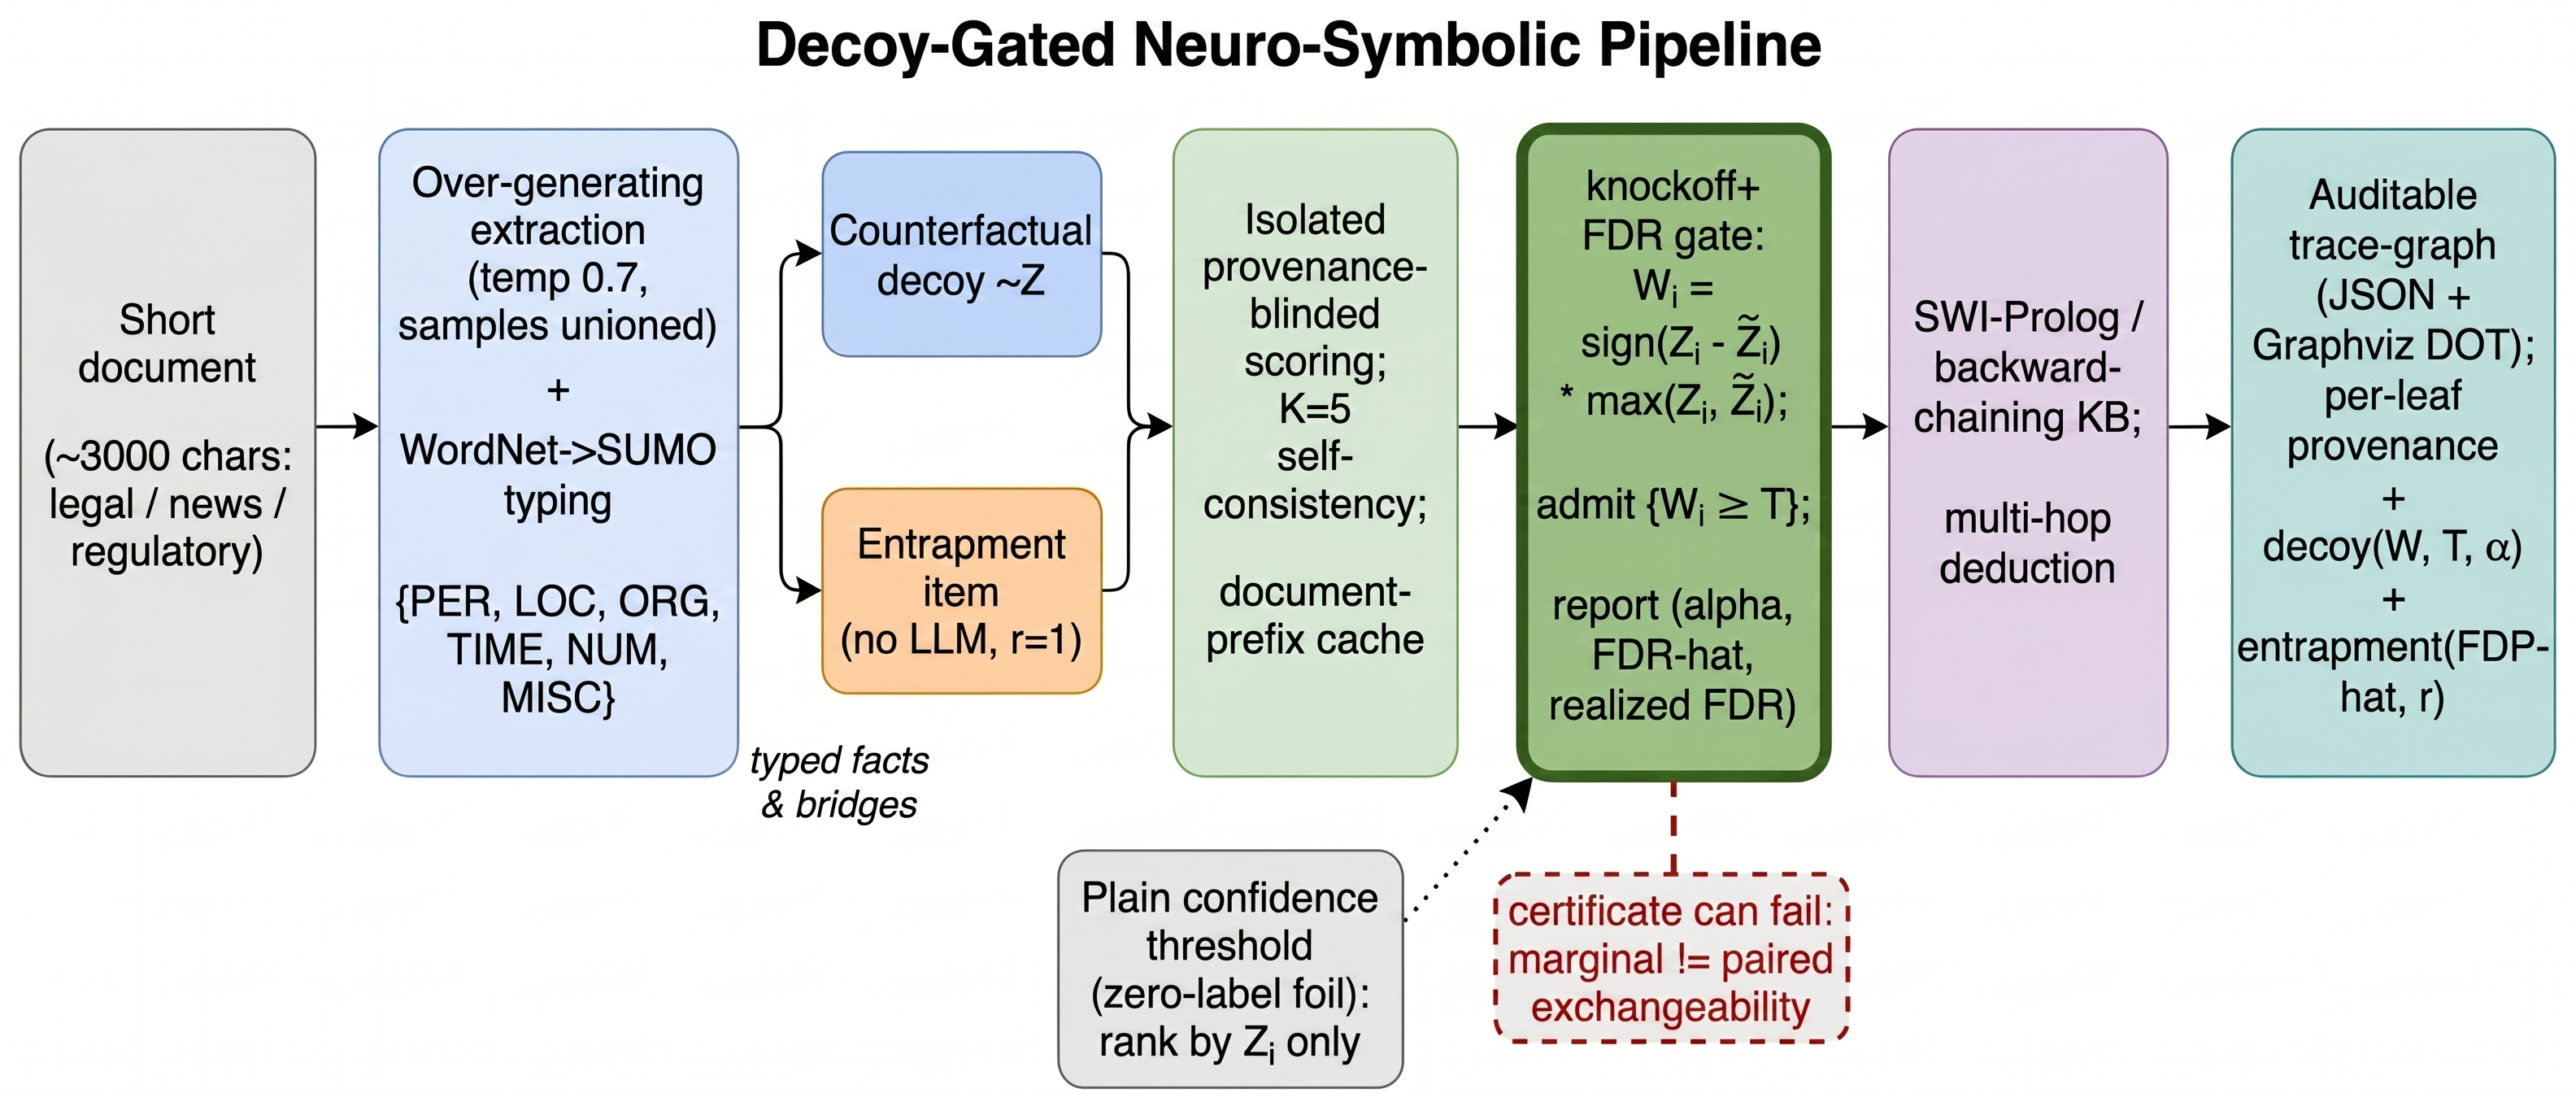
\includegraphics[width=\linewidth,height=0.4\textheight,keepaspectratio]{figures/fig1_v0.jpg}
  \caption{End-to-end decoy-gated text-to-logic pipeline. A short document is over-generated into typed first-order facts and bridges; each candidate is paired with a plausibility-matched counterfactual decoy and an independently-built entrapment item; an isolated, provenance-blinded self-consistency elicitation scores all of them; the knockoff+ gate admits candidates with $W_i \ge T$ at the most permissive target whose estimated FDR is $\le\alpha$; admitted facts populate a backward-chaining knowledge base that emits a trace-graph whose every leaf carries provenance, decoy $(W_i,T,\alpha)$, and entrapment $(\widehat{\mathrm{FDP}},r)$ certificates.}
  \label{fig:pipeline}
\end{figure}

What makes this informative rather than merely negative is \emph{why} it happens, and we localize the cause precisely. Self-consistency \emph{does} restore the property the diagnostic measures: the counterfactual-decoy score distribution is statistically indistinguishable from the model's own spontaneous errors (full-distribution KS $p=0.058$; admission-tail KS $p=0.31$; both fail to reject) and sharply distinct from true positives (KS $p=5\times10^{-9}$). That is \emph{marginal} (distributional) exchangeability. The knockoff+ gate, however, needs the \emph{per-pair} sign-flip property at the cutoff, and it fails: among the twelve admitted multi-hop reals, the model scored each false real \emph{above} its own matched decoy. Distributional exchangeability is necessary but not sufficient for paired exchangeability---and the win-rate diagnostic, being a marginal statistic, cannot see the gap. This two-layer decomposition is, we argue, the generalizable lesson of transplanting knockoffs to LLM scoring.

The same rigor is then applied where the goal actually lives. We \emph{execute} the previously-missing application headline on a genre-faithful 24-document legal/news/regulatory anchor\footnote{Code: \url{https://github.com/AMGrobelnik/ai-invention-6db730-decoy-gated-neuro-symbolic-extraction-a/tree/main/round-3/experiment-2}}: the operational pipeline ingests $\sim$3000-character documents, types entities against an upper ontology, gates extracted facts, runs multi-hop deductions, and emits auditable trace-graphs whose every leaf carries a provenance span and the decoy and entrapment certificates that licensed it. Here the gate behaves better than on the hard CLUTRR family---its self-report is \emph{conservative}, it cuts the corrupted multi-hop conclusion rate from $0.48$ to $0.18$, and it reduces the atomic hallucination rate by $\sim 25\%$ (directional; bootstrap CIs overlap at $n{=}24$). Finally, on $152$ Re-DocRED documents the operational wedge over plain thresholding is disconfirmed at recall $\le0.075$, and we recast the operational contribution as a \emph{gold-free regime-diagnostic} that predicts that null result without labels (prediction correct).

\paragraph{Summary of contributions.}
\begin{itemize}
  \item We formulate the \emph{text-to-logic admission boundary} as an FDR-control problem and introduce \emph{decoy-gated extraction}, to our knowledge the first label-free FDR knob at the neural-to-symbolic interface, built from a single canonical knockoff+ statistic, plausibility-matched counterfactual decoys, and independent entrapment corroboration (Sections 3--4).
  \item We answer the central methodology objection by re-running the calibration diagonal under the diagnostic-validated self-consistency elicitation, and report the pre-registered disconfirmation honestly: the gate does not control FDR on the populable multi-hop family (Section 6.1).
  \item We isolate the mechanism---\emph{marginal decoy exchangeability does not imply paired sign-flip exchangeability} at the cutoff---and show the win-rate diagnostic, being marginal, over-predicts gate validity, a fundamental blind spot we report rather than paper over (Sections 6.2--6.3).
  \item We \emph{execute} the genre-faithful application headline the prior draft was missing: a quantified, regime-mapped hallucination-reduction run on 24 professional documents with exported auditable trace-graphs, including a multi-hop corruption drop from $0.48$ to $0.18$ (Section 6.4).
  \item We scale the Re-DocRED operational test to its true scope (152 documents, recall $\le0.075$, all comparators participating, powered multi-hop comparison) and contribute a novel \emph{label-free regime-diagnostic} that forecasts the gate's null wedge gold-free (Section 6.5).
\end{itemize}

\section{Related Work}

\paragraph{Label-free hallucination scoring.} Zero-resource detectors produce per-claim hallucination scores from sampling consistency (SelfCheckGPT \cite{Manakul2023}) or distractor-normalized verbalized confidence (DINCO \cite{Wang2025}); FactSelfCheck \cite{Sawczyn2025} operates natively at the fact level over $(h, r, t)$ triples. These methods yield a \emph{score}, not an admission threshold, and offer no exchangeability or competition argument. In our framework they are \emph{candidate elicitations} feeding the gate, not the gate itself, and we select among them by \emph{tail} behavior. Verbalized confidence is known to be overconfident in the upper tail \cite{Xiong2023}, and token log-probability calibration degrades under reinforcement learning from human feedback \cite{Tian2023}---two facts our results turn from caveats into a measured, central phenomenon.

\paragraph{Labeled uncertainty quantification for LLMs.} Conformal factuality \cite{Mohri2024} removes claims until a factuality level is met, using a labeled calibration set, and certifies the emitted answer; coherent factuality \cite{RubinToles2025} extends this to reasoning chains; conformal selection \cite{Jin2022}, multiple-testing hallucination detection \cite{Li2025}, and online/feedback-driven testing \cite{Lu2025} control FDR over candidate outputs but require labeled calibration outcomes; conformal e-value novelty detection \cite{Bashari2023} and conformal link prediction \cite{Marandon2023} control FDR over selected test points or predicted edges under (adapted) exchangeability of a labeled reference set. Table~\ref{tab:novelty} contrasts the closest neighbors. Every one is \emph{labeled} and certifies a \emph{model output} under assumed exchangeability; ours is \emph{label-free}, targets an \emph{intermediate admission boundary}, manufactures the null behavior with engineered-and-tested decoys, and---crucially---empirically \emph{tests} the exchangeability that the others assume\footnote{Code: \url{https://github.com/AMGrobelnik/ai-invention-6db730-decoy-gated-neuro-symbolic-extraction-a/tree/main/round-2/research-1}}. The distinction defuses the natural rebuttal that decoy-gating ``is just conformal selection at the fact level'': conformal selection imports exchangeability from a labeled calibration set whose outcomes are observed, whereas we have zero such labels and must test the fair-coin sign-flip property in the score tail---and we find that it can fail.

\begin{table}[t]
\centering
\small
\begin{tabular}{lcccc}
\toprule
Method & Labels? & Unit certified & Decoy? & Controls \\
\midrule
Conformal selection \cite{Jin2022} & Yes & output shortlist & No & FDR \\
Multiple-testing hallucination \cite{Li2025} & Yes & generation & No & FDR \\
Conformal e-value novelty \cite{Bashari2023} & Yes & test points & No & FDR \\
Conformal link prediction \cite{Marandon2023} & Yes & predicted edges & No & FDR \\
Conformal factuality \cite{Mohri2024} & Yes & emitted claims & No & coverage \\
\textbf{Decoy-gating (ours)} & \textbf{No} & \textbf{admission boundary} & \textbf{Yes} & \textbf{FDR (tested)} \\
\bottomrule
\end{tabular}
\caption{Decoy-gating against its nearest FDR/conformal neighbors. All prior methods require labeled calibration and certify a model output under assumed exchangeability; ours is label-free, targets the intermediate text-to-logic admission, and empirically tests an engineered decoy sign-flip property---which we show is elicitation-dependent and can break even when its marginal proxy holds.}
\label{tab:novelty}
\end{table}

\paragraph{FDR control by competition.} The knockoff filter \cite{Barber2015} and Model-X knockoffs \cite{Cands2016} select signals with guaranteed FDR by competing each real candidate against a synthetic negative control exchangeable by construction, relying on the null sign-flip property; the knockoff+ threshold controls FDR exactly via the conservative $+1$ offset \cite{Barber2015}, which Rajchert and Keich prove is in general necessary \cite{Rajchert2022}. Ebadi et al. give tighter upper prediction bounds on the FDP \cite{Ebadi2023}. In proteomics, entrapment estimation provides an independent FDP bound, with the valid combined estimator and the flawed naive estimator characterized by Wen et al. \cite{Wen2024}; property-matched decoy generation (DeepCoy \cite{Imrie2020}) shows decoys must reproduce a target score distribution. We adapt all three to the LLM boundary, where exchangeability is \emph{not} provable. Our contribution to this line is empirical and cautionary: we show that at the LLM boundary the construction can satisfy the \emph{marginal} matching DeepCoy targets while still violating the \emph{paired} sign-flip property the knockoff theorems require.

\paragraph{Text-to-logic neuro-symbolic reasoning.} LINC \cite{Olausson2023} and Logic-LM \cite{Pan2023} semantic-parse premises into first-order logic or symbolic programs executed by a solver, with majority voting or solver-error self-refinement; LLM-ASP \cite{Yang2023} parses CLUTRR into reusable answer-set modules. None exercises principled control over \emph{which} extracted premises are admitted: a syntactically valid but fabricated premise is never challenged, voting merely smooths variance, and refinement fixes only solver and syntax errors. Standard neural baselines---chain-of-thought prompting \cite{Wei2022} and retrieval-augmented generation \cite{Lewis2020}---have no admission boundary at all. Logical-reasoning benchmarks such as RuleTaker \cite{Clark2020}, ProofWriter \cite{Tafjord2020}, and CLUTRR \cite{Sinha2019} supply controlled targets; our calibration anchor is CLUTRR for its crisp templated gold, and our operational anchor is Re-DocRED \cite{Tan2022}, the false-negative-corrected re-annotation of DocRED \cite{Yao2019}. For the symbolic layer we type arguments with WordNet \cite{Miller1995} anchored to the SUMO upper ontology \cite{Niles2001}, and design a probabilistic upgrade on ProbLog \cite{Raedt2007}, whose DeepProbLog extension \cite{Manhaeve2018} is the precedent for an external model supplying clause probabilities.

\section{Preliminaries}

We control the false admission of two candidate kinds. A \emph{fact} is a ground typed atom (for example \texttt{rel\_child(e\_alice, e\_bob)}), and a \emph{bridge} is a fuzzy-unification rule---a kinship composition rule for CLUTRR, or a surface-form-to-schema relation alignment for the open-vocabulary anchors. Bridges are first-class admission candidates with their own decoy, score, and gate.

\paragraph{The canonical competition statistic.} Each candidate $i$ receives a label-free score $Z_i$ from an isolated elicitation and a matched decoy score $\tilde{Z}_i$. We use a single statistic throughout: the knockoff+ \emph{signed maximum}
$$W_i = \operatorname{sign}(Z_i - \tilde{Z}_i)\cdot\max(Z_i, \tilde{Z}_i),$$
whose magnitude is the larger of the two scores and whose sign records which won. A large positive $W_i$ is evidence that the candidate is a true signal. The per-pair \emph{signed difference} $d_i = Z_i - \tilde{Z}_i$ is used \emph{only} as a measurement-only tail diagnostic (win-rate and CDF tests), never as the gating statistic.

\paragraph{Two notions of exchangeability, and why the distinction is load-bearing.} Knockoff+ delivers a finite-sample FDR guarantee only under the \emph{paired sign-flip property}: among genuinely false candidates, $\operatorname{sign}(W_i)$ is an independent fair coin conditional on $|W_i|$, i.e.\ a false real and its matched decoy are equally likely to take the larger score \emph{as a pair}. A strictly weaker, and separately measurable, property is \emph{marginal (distributional) exchangeability}: the pooled distribution of decoy scores equals the pooled distribution of false-real scores. DeepCoy-style decoy design \cite{Imrie2020} and the win-rate / CDF diagnostics target the \emph{marginal} property. Our central empirical finding (Section 6.2) is that the two come apart at the LLM boundary: self-consistency restores the marginal property while the paired property still fails, so the marginal diagnostic over-certifies the gate.

\paragraph{The targets and the two roles of resampling.} The target is the corpus-aggregate FDR---the expected fraction of admitted candidates that are document-non-entailed---held at or below a user-chosen $\alpha$, separately for facts and bridges and per anchor. We report, for every certified cell, the \emph{triple} $(\alpha,\ \widehat{\mathrm{FDR}},\ \text{realized FDR})$, so that a gate whose own estimate $\widehat{\mathrm{FDR}}$ undershoots the realized FDR is flagged as \emph{self-report anti-conservative} even when the realized FDR happens to land below $\alpha$. The \emph{document-block bootstrap} (resampling whole documents, $B = 2000$ \cite{Cameron2008}) supplies confidence intervals on the realized FDP and a within-document-dependence diagnostic; it quantifies sampling variability and does \emph{not} restore the guarantee under dependence. Because the conservative $+1$ makes the smallest attainable estimate $1/k$ with $k$ admissions, certifying $\widehat{\mathrm{FDR}}\le\alpha$ requires $k \ge \lceil 1/\alpha \rceil$; the demonstrable grid $\alpha\in\{0.05,0.1,0.2,0.3,0.5\}$ maps to admission floors $\{20,10,5,4,2\}$, and any $\alpha$ below an anchor's reachable floor is reported as structurally undemonstrable, never as ``confirmed by conservatism.''

\section{Method}

The pipeline has six stages: over-generating extraction, plausibility-matched decoy generation, isolated provenance-blinded scoring, the knockoff+ FDR gate, independent entrapment corroboration, and symbolic reasoning with auditable trace-graphs. The full implementation specification---verbatim prompt templates, on-disk formats, and library APIs---is provided in the supporting research artifacts\footnote{Code: \url{https://github.com/AMGrobelnik/ai-invention-6db730-decoy-gated-neuro-symbolic-extraction-a/tree/main/round-1/research-1}}\footnote{Code: \url{https://github.com/AMGrobelnik/ai-invention-6db730-decoy-gated-neuro-symbolic-extraction-a/tree/main/round-1/research-2}}.

\subsection{Extraction with deliberate over-generation}

A cheap LLM proposes typed first-order facts and bridges from the document in a LINC/Logic-LM style \cite{Olausson2023, Pan2023}, with argument types grounded in a commodity upper-ontology slice. Because OpenCyc was discontinued by Cycorp in March 2017 and survives only as unmaintained mirrors, and ResearchCyc is license-gated, OpenCyc cannot be a reproducible commodity dependency; we substitute an offline WordNet \cite{Miller1995} hypernym lookup that maps each argument head noun into the coarse vocabulary $\{$PER, LOC, ORG, TIME, NUM, MISC$\}$ via anchor synsets, each coarse type further anchored to a SUMO upper-ontology class (e.g.\ \texttt{person.n.01} $\to$ PER $\to$ \texttt{\&\%Human}) \cite{Niles2001}. Typing is used \emph{only} to constrain decoy generation and entity linking, never to filter; because it never rejects a candidate it cannot break the FDR guarantee. The extractor deliberately \emph{over-generates} (temperature $0.7$, multiple samples unioned) so the candidate pool is dense in genuine false positives---a precondition for a non-vacuous calibration diagonal.

\subsection{Plausibility-matched counterfactual decoys}

The load-bearing design choice is the decoy family. The relevant target distribution at the LLM boundary is not the true-positive distribution DeepCoy matches in molecular screening \cite{Imrie2020}, but the distribution of the model's \emph{own spontaneous false extractions}---the plausible hallucinations the gate must actually catch. Our primary family is the \emph{document-conditioned counterfactual}: given the document and the relation/type schema, the model produces a maximally plausible fact or bridge that is \emph{not} entailed by the text, matching the surface form and specificity of the document's real facts. Every decoy passes an independent isolated non-entailment check (an accidentally entailed decoy is actually true and would bias the FDR conservatively); the contamination rate is logged (CLUTRR $8.4\%$, application anchor $5.7\%$). As a deliberately retained negative control we also generate \emph{random type-matched swaps}, predicted to read anti-conservative precisely because they are too easy. Crucially, we do not assume the decoys match the spontaneous-error distribution---we \emph{test} it (Section 6.2), and, as the same section shows, we test whether marginal matching is sufficient.

\subsection{Isolated, provenance-blinded scoring and elicitation selection}

Each candidate---real, decoy, or entrapment---is scored in its \emph{own} prompt with source identity masked and presentation order randomized, removing within-batch contrast effects that would let the model implicitly detect a fabricated item and depress its score. Document-prefix prompt caching makes isolated scoring affordable. The per-candidate score is produced by a \emph{tail-exchangeability}-selected elicitation, not an average-calibration-selected one. This selection criterion is the key correction over the prior draft: a Phase-0 pilot ranks verbalized confidence, a DINCO-style distractor-normalized score \cite{Wang2025}, a $K$-sample self-consistency score \cite{Manakul2023, Sawczyn2025}, and a log-probability yes/no score by their \emph{tail} decoy win-rate (target $\approx 0.5$), not by full-distribution AUC. The distinction matters because the two criteria disagree: verbalized confidence and DINCO have higher full-distribution AUC ($0.861$ and $0.871$) yet fail the tail test, whereas $K{=}5$ self-consistency has the tail win-rate that covers $0.5$ ($0.482$)\footnote{Code: \url{https://github.com/AMGrobelnik/ai-invention-6db730-decoy-gated-neuro-symbolic-extraction-a/tree/main/round-2/experiment-2}}. Higher AUC does not imply tail-exchangeability; self-consistency therefore hosts the headline diagonal. The generator$\neq$scorer ablation that de-circularizes the construction is settled (Section 6.3) and carried forward.

\subsection{The knockoff+ FDR gate and its self-report}

Given the competition statistics, the gate admits $\{i : W_i \ge T\}$ at the smallest cutoff $T$ for which $\widehat{\mathrm{FDR}}(T) \le \alpha$ \cite{Barber2015}. We keep the conservative $+1$ for the headline certificate. Beyond realized FDR (against gold) and the target $\alpha$, we \emph{always} report the gate's internal estimate $\widehat{\mathrm{FDR}}$, so that the failure mode ``the estimate is anti-conservative'' ($\widehat{\mathrm{FDR}} < \text{realized}$) is surfaced as its own disconfirmation even when realized FDR lands below $\alpha$.

\subsection{Independent entrapment corroboration}

Decoy competition decides admission; \emph{entrapment} provides an independent upper bound on the realized FDP, built by a mechanism \emph{distinct} from the decoys (in-genre cross-document swaps, numeric or temporal perturbation, explicit contradiction) and constructed \emph{without} the generating LLM. We use the valid combined estimator $\widehat{\mathrm{FDP}} = N_E(1 + 1/r)/(N_T + N_E)$ as the default certificate \cite{Wen2024}, with $N_T,N_E$ the admitted target and entrapment counts and $r$ the entrapment-to-target ratio; we never use the naive estimator, which Wen et al. prove biased \cite{Wen2024}.

\subsection{Symbolic reasoning and auditable trace-graphs}

Admitted facts and bridges populate a backward-chaining knowledge base for multi-hop deduction; we target SWI-Prolog through the \texttt{janus-swi} bridge and fall back to a pure-Python meta-interpreter with an identical trace-graph schema when the native bridge is unavailable. A \texttt{solve/2}-style meta-interpreter captures the proof as a \emph{trace-graph} whose nodes are sub-goals and derived facts and whose edges are labeled rule applications. Every leaf resolves to a certificate term: the provenance span, the decoy-competition certificate $(W_i, T, \alpha)$, and the entrapment certificate $(\widehat{\mathrm{FDP}}, r)$. The trace-graph serializes to JSON for machine audit and Graphviz DOT for human audit. A designed \emph{probabilistic} upgrade swaps the deterministic query for ProbLog's \texttt{get\_evaluatable().evaluate()} \cite{Raedt2007}, turning each admitted clause into a weighted clause $p_i :: \mathrm{fact}$ with $p_i$ a calibrated function of $Z_i$, so derived conclusions carry marginal probabilities while every leaf retains its certificate.

\section{Experimental Setup}

The evaluation is split so that calibration and operational usefulness are proven on the data each suits, and the protocol is pre-registered so every outcome---confirmed, disconfirmed, or untestable---is interpretable.

\subsection{Three anchors with a clean division of labor}

CLUTRR \cite{Sinha2019} is rule-based and templated, so its kinship gold is exact---the property that lets it host the realized-FDR-versus-$\alpha$ \emph{diagonal} and the single primary disconfirmation. The corpus draws on a standardized atomic + multi-hop kinship triple set derived entirely from CLUTRR's own \texttt{proof\_state} fields over a 20-relation vocabulary\footnote{Code: \url{https://github.com/AMGrobelnik/ai-invention-6db730-decoy-gated-neuro-symbolic-extraction-a/tree/main/round-1/dataset-1}}; the diagonal in this paper is computed on the error-dense $40$-document checkpoint of the scaled confirmatory split, which yields $410$ extracted reals ($123$ true, $287$ spontaneous false) and is populable on both families ($129$ false atomic, $158$ false multi-hop, exceeding the pre-registered $N_{\text{false\_min}}=40$ floor). Re-DocRED \cite{Tan2022} is human-annotated, open-vocabulary, and document-level, so it hosts the \emph{operational} comparison and the genuine schema-alignment bridge test; the anchor comprises Wikipedia documents with gold $(head, relation, tail)$ triples over $96$ Wikidata relations\footnote{Code: \url{https://github.com/AMGrobelnik/ai-invention-6db730-decoy-gated-neuro-symbolic-extraction-a/tree/main/round-1/dataset-2}}, and because it retains residual false negatives it licenses only \emph{relative} operational comparisons. Finally, the genre-faithful \emph{application anchor} is $24$ genuine professionally-written documents ($8$ legal, $8$ news, $8$ regulatory; native length $1239$--$3474$ characters, mean $2372$, squarely in the $\sim$3000-character target range), standardized to the same triple schema with character-span provenance and $140$ human/structure-derived gold facts built with no LLM in the loop\footnote{Code: \url{https://github.com/AMGrobelnik/ai-invention-6db730-decoy-gated-neuro-symbolic-extraction-a/tree/main/round-2/dataset-1}}. CLUTRR tests whether the knob is calibrated; the application anchor tests whether it reduces hallucination on the documents the goal targets; Re-DocRED tests whether it beats plain thresholding operationally.

\subsection{Pipeline, baselines, and metrics}

All systems run on commodity CPU with \texttt{openai/gpt-4.1-nano} via OpenRouter as the primary model and \texttt{mistralai/ministral-8b-2512} as the cross-family scorer/adjudicator. The comparators are the \emph{plain confidence-threshold gate} (the primary zero-label foil, identical elicitation, no decoy or competition), chain-of-thought \cite{Wei2022}, retrieval-augmented generation \cite{Lewis2020}, and labeled Mohri--Hashimoto conformal factuality \cite{Mohri2024}. On Re-DocRED a single fixed claim-decomposition and relation-alignment step maps every system's raw output into the shared triple space identically (a MiniLM \cite{Reimers2019} top-eight relation shortlist followed by a temperature-0 pick among the 96 codes, with three-tier entity linking), and recall is matched by sweeping each system's own score to a common operating point. All confidence intervals use the document-block bootstrap and all multiplicity is controlled by Benjamini--Hochberg at $q = 0.05$.

\subsection{Pre-registered claims and the primary disconfirmation}

Table~\ref{tab:claims} lists the pre-registered claim chain and its verdicts. The single primary disconfirmation is fixed in advance: on the populable CLUTRR family (default multi-hop) under isolated \emph{self-consistency} scoring at the operative $\alpha^{*}$, the central control claim is disconfirmed if realized FDR exceeds $\alpha^{*}+\tau$ (with $\tau=0.05$) and the document-block CI lies entirely on the anti-conservative side; additionally the gate's self-report is disconfirmed if $\widehat{\mathrm{FDR}}$ is anti-conservative relative to realized FDR.

\begin{table}[t]
\centering
\small
\begin{tabular}{lll}
\toprule
Claim & Test & Verdict \\
\midrule
S0 Score separation & tail-exchangeability selection (not AUC) & PASS \\
S1 Marginal decoy match & decoy$\approx$spont (KS $p{=}0.058$), $\neq$ true-pos & PASS \\
S1b Diagnostic sensitivity & swap control loses sensitivity; ladder underpowered & FAIL (blind spot) \\
S2 Calibration diagonal & multi-hop realized FDR $1.0$ at $\alpha^{*}{=}0.5$ & DISCONFIRMED \\
S2-self & $\widehat{\mathrm{FDR}}{=}0.5 <$ realized $1.0$ & DISCONFIRMED \\
S2b Generator$\neq$scorer & 4/4 configs win-rate CI covers $0.5$ & ROBUST \\
S3 Entrapment & $\widehat{\mathrm{FDP}}$ high at $\alpha{=}0.5$ (loose admit) & AGREES (loosely) \\
S4 Operational wedge & $\Delta$(METHOD$-$PLAIN)$\le0$ at recall $\le0.075$ & DISCONFIRMED \\
S4b Application headline & corruption $0.48{\to}0.18$; atomic $-25\%$ (CI overlap) & EXECUTED \\
\bottomrule
\end{tabular}
\caption{Pre-registered claim-chain verdicts under the diagnostic-validated self-consistency elicitation. The calibration certificate (S2) is honestly disconfirmed; the marginal decoy match (S1) holds, which is exactly what makes S2 instructive; the operational pipeline (S4b) delivers a measured corruption reduction and auditable traces.}
\label{tab:claims}
\end{table}

\section{Results}

We lead with the corrected calibration diagonal, explain its disconfirmation mechanistically, then report the executed application headline and the reframed operational wedge.

\subsection{The corrected CLUTRR calibration diagonal under self-consistency (S2)}

Re-running the headline diagonal under the diagnostic-validated $K{=}5$ self-consistency elicitation reverses the prior draft's claim. On the error-dense multi-hop family---the pre-registered populable family, $\sim 85\%$ genuine false because the extractor's forced multi-hop relation accuracy is only $0.17$---the gate certifies admissions at exactly one target, $\alpha^{*}=0.5$ (the $1/k$ floor blocks all stricter $\alpha$). At that target the realized FDR against crisp gold is $1.0$: of $12$ admitted reals, all $12$ are document-non-entailed, with document-block CI $[0.66,1.0]$ lying entirely above $\alpha^{*}$. The gate's own self-report $\widehat{\mathrm{FDR}}=0.5$ undershoots the realized $1.0$. The pre-registered primary disconfirmation therefore \emph{fires} on both the calibration and the self-report criteria.

\begin{figure}[!htbp]
  \centering
  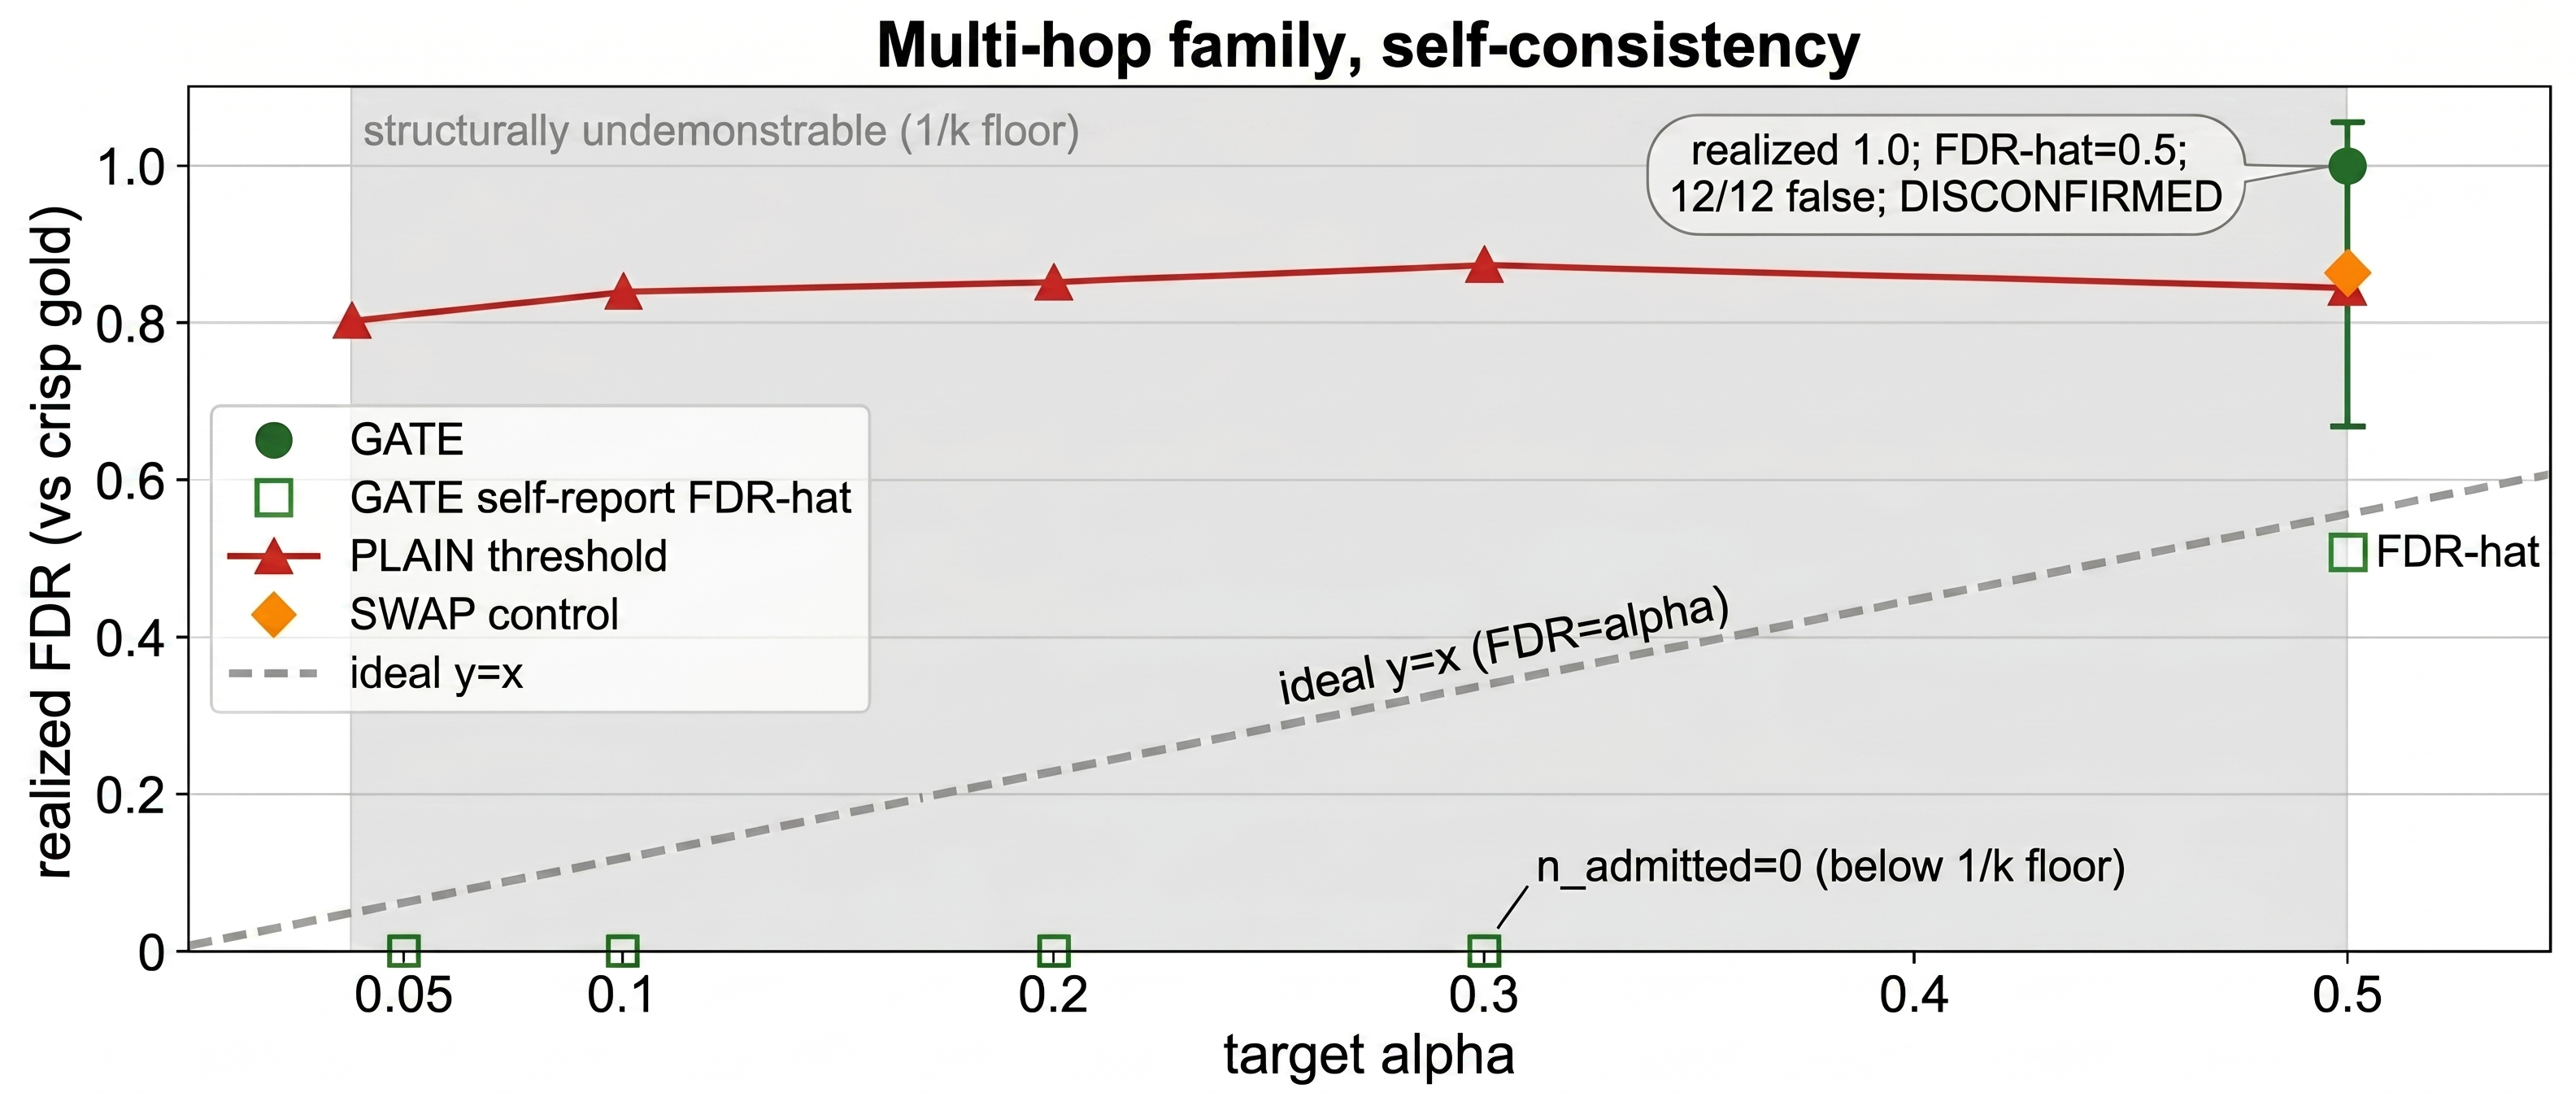
\includegraphics[width=\linewidth,height=0.4\textheight,keepaspectratio]{figures/fig2_v0.jpg}
  \caption{Realized FDR versus target $\alpha$ on the populable CLUTRR multi-hop family under the diagnostic-validated K=5 self-consistency elicitation. The knockoff+ gate certifies admissions only at $\alpha^{*}=0.5$ (the $1/k$ floor blocks stricter targets); there realized FDR is $1.0$ (12/12 admitted are false), with document-block-bootstrap CI $[0.66,1.0]$ lying entirely above $\alpha^{*}$, and the gate's own self-report $\widehat{\mathrm{FDR}}=0.5$ undershoots it. The pre-registered primary disconfirmation fires. The plain threshold and swap-decoy baselines are worse still.}
  \label{fig:diagonal}
\end{figure}

The atomic family tells the same story more mildly: at $\alpha=0.3$ realized FDR is $0.377$ (61 admitted, 23 false) against a self-report of $0.279$---a target violation ($0.377>0.3$) and an anti-conservative self-report---while at $\alpha=0.5$ realized FDR is $0.422$ with self-report $0.491$ (within target). Across both families the plain confidence-threshold baseline is worse still (multi-hop realized FDR $0.80$--$0.87$; atomic $0.17$--$0.55$), so decoy competition \emph{helps relative to plain thresholding} even here---but ``better than an uncontrolled baseline'' is not ``controls FDR at $\alpha$,'' and we do not claim the latter. The prior draft's apparent conservatism\footnote{Code: \url{https://github.com/AMGrobelnik/ai-invention-6db730-decoy-gated-neuro-symbolic-extraction-a/tree/main/round-2/experiment-1}} is, when the same verbalized elicitation is re-run on this data, a discreteness/loose-target artifact: the verbalized diagonal admits \emph{nothing} on the multi-hop family at any $\alpha$ and violates the target on the atomic family at $\alpha=0.5$ (realized $0.534>0.5$, self-report $0.5$). We therefore retain verbalized only as a documented contrast, never as a co-headline.

\subsection{Why the gate fails: marginal vs.\ paired exchangeability (S1)}

The disconfirmation is informative because the marginal precondition the diagnostic checks \emph{does} hold under self-consistency. The counterfactual-decoy score distribution is statistically indistinguishable from the model's own spontaneous-error distribution---full-distribution KS $p=0.058$, Mann--Whitney $p=0.061$, Anderson--Darling $p=0.061$, permutation $p=0.060$ (all fail to reject), tightening in the admission tail (top-25\% KS $p=0.31$)---and sharply distinct from the true-positive distribution (KS $p=5\times10^{-9}$, Mann--Whitney $p=4\times10^{-12}$). By the marginal criterion the decoys are exactly right: they look like the spontaneous errors, not like the true facts.

\begin{figure}[!htbp]
  \centering
  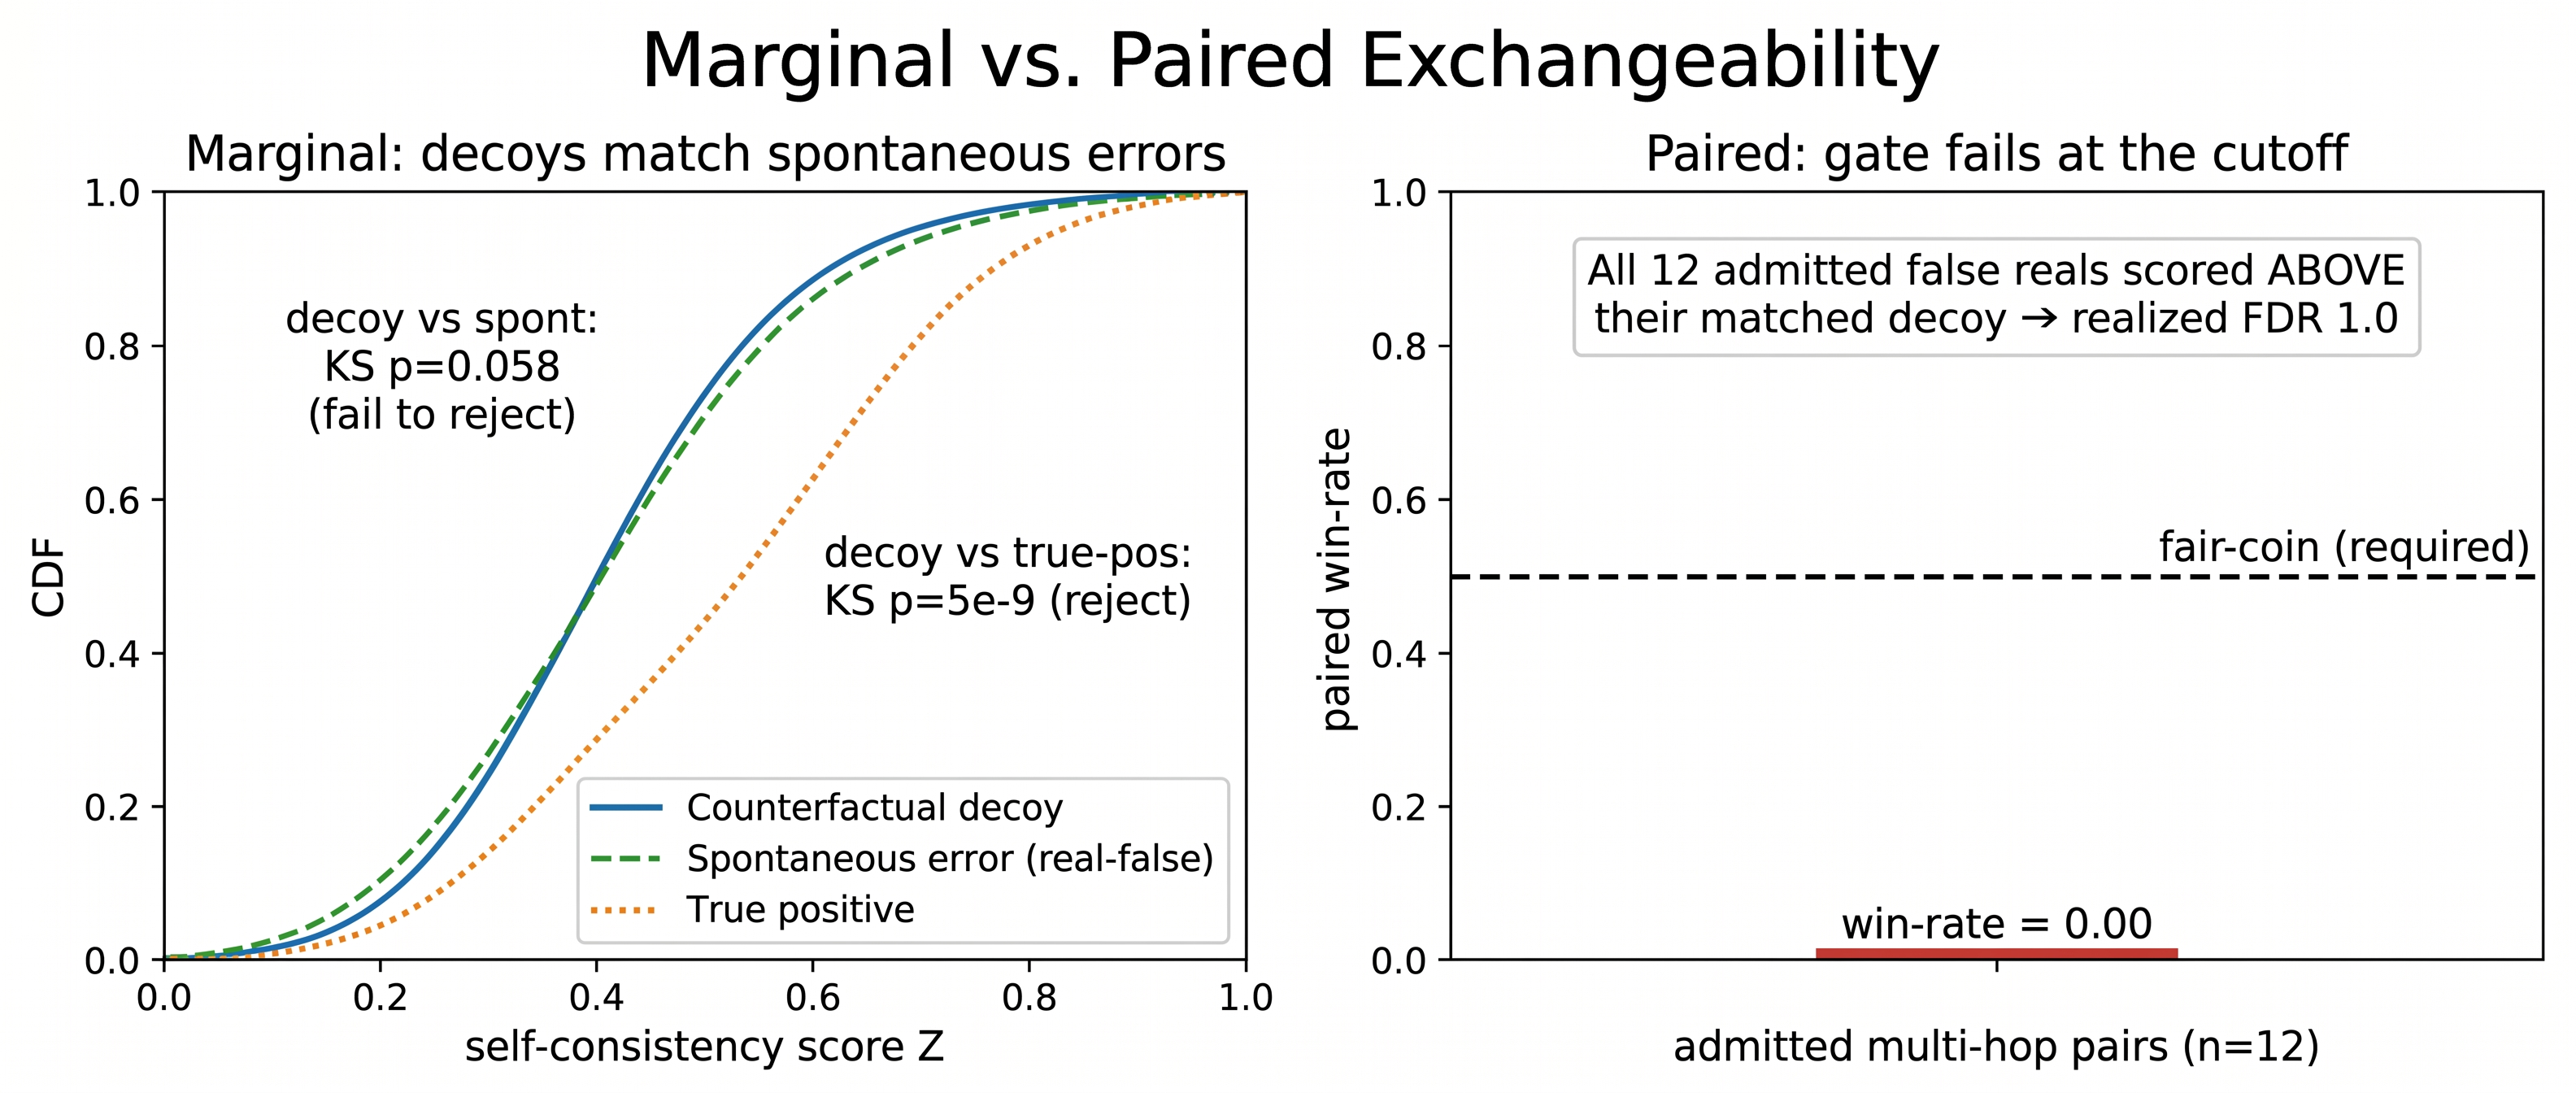
\includegraphics[width=\linewidth,height=0.4\textheight,keepaspectratio]{figures/fig3_v0.jpg}
  \caption{The disconfirmation localized. Left: pooled score CDFs under self-consistency---the counterfactual decoy distribution is statistically indistinguishable from the model's own spontaneous errors (full KS $p=0.058$; tail KS $p=0.31$) and sharply distinct from true positives (KS $p=5\times10^{-9}$), so the \emph{marginal} exchangeability the win-rate diagnostic checks holds. Right: at the admission cutoff the \emph{paired} competition fails---all 12 admitted multi-hop reals out-score their own matched decoy (paired win-rate $0\%$), the property knockoff+ actually requires. Marginal exchangeability does not imply paired exchangeability.}
  \label{fig:exchange}
\end{figure}

Yet the paired competition fails. Among the twelve admitted multi-hop reals, the model assigned each false real a \emph{higher} self-consistency score than its own matched decoy---the per-pair sign-flip property knockoff+ requires is violated precisely in the admission tail where it matters. The reconciliation is that marginal (distributional) exchangeability is strictly weaker than paired exchangeability: two pooled distributions can coincide while, pair by pair, the false real systematically out-scores its decoy. This gap is the generalizable lesson. Property-matched decoy design and win-rate/CDF diagnostics, imported from cheminformatics and proteomics, certify the \emph{marginal} property; the knockoff theorems need the \emph{paired} one; at the LLM boundary the two come apart, and a marginal diagnostic cannot detect the difference. We state this as a limitation of the entire decoy-competition approach to LLM fact admission, not of one elicitation.

\subsection{The diagnostic blind spot and de-circularization (S1b, S2b)}

The blind spot has a second, independently measured face. Under the very $K{=}5$ self-consistency that restores marginal exchangeability, the random-swap negative control---which \emph{must} read anti-conservative---is no longer reliably flagged: at this checkpoint the difficulty ladder L0--L4 is underpowered (only two false pairs reach the operative tail per rung), and its verdict is \texttt{PARTIAL}---the diagnostic detects only grossly out-of-context (foreign-entity) decoys and loses resolution for in-distribution rungs. Combined with the marginal-vs-paired gap, this means the win-rate diagnostic both (i) over-predicts paired validity and (ii) loses sensitivity to too-easy decoys in the regime where it is supposed to be trusted. We therefore \emph{downgrade} the prior draft's ``the diagnostic tells the practitioner which regime they are in'' claim to ``the diagnostic detects gross non-exchangeability and tail-overconfidence but cannot certify paired validity,'' and we mark a sensitive paired-exchangeability diagnostic as required future work.

The one circularity concern that \emph{is} settled is shared-model bias. The generator$\neq$scorer ablation is robust: across all four $(G,S)$ configurations---including decoys generated by gpt-4.1-nano and scored by the cross-family ministral-8b, and the symmetric swap---the tail win-rate CI covers $0.5$ (e.g.\ $0.491$, CI $[0.37,0.61]$, KS $p=0.999$). The marginal exchangeability self-consistency restores is therefore not an artifact of one model scoring its own outputs; the \emph{paired} failure is likewise not a circularity artifact but a genuine property of LLM tail scoring.

\subsection{The application headline: hallucination reduction and auditable traces (S4b)}

We then execute the genre-faithful application run the prior draft was missing, on the 24-document legal/news/regulatory anchor, reporting both elicitations across the full $\alpha$ grid so the regime-dependence is never obscured. Three honest findings follow.

\begin{figure}[!htbp]
  \centering
  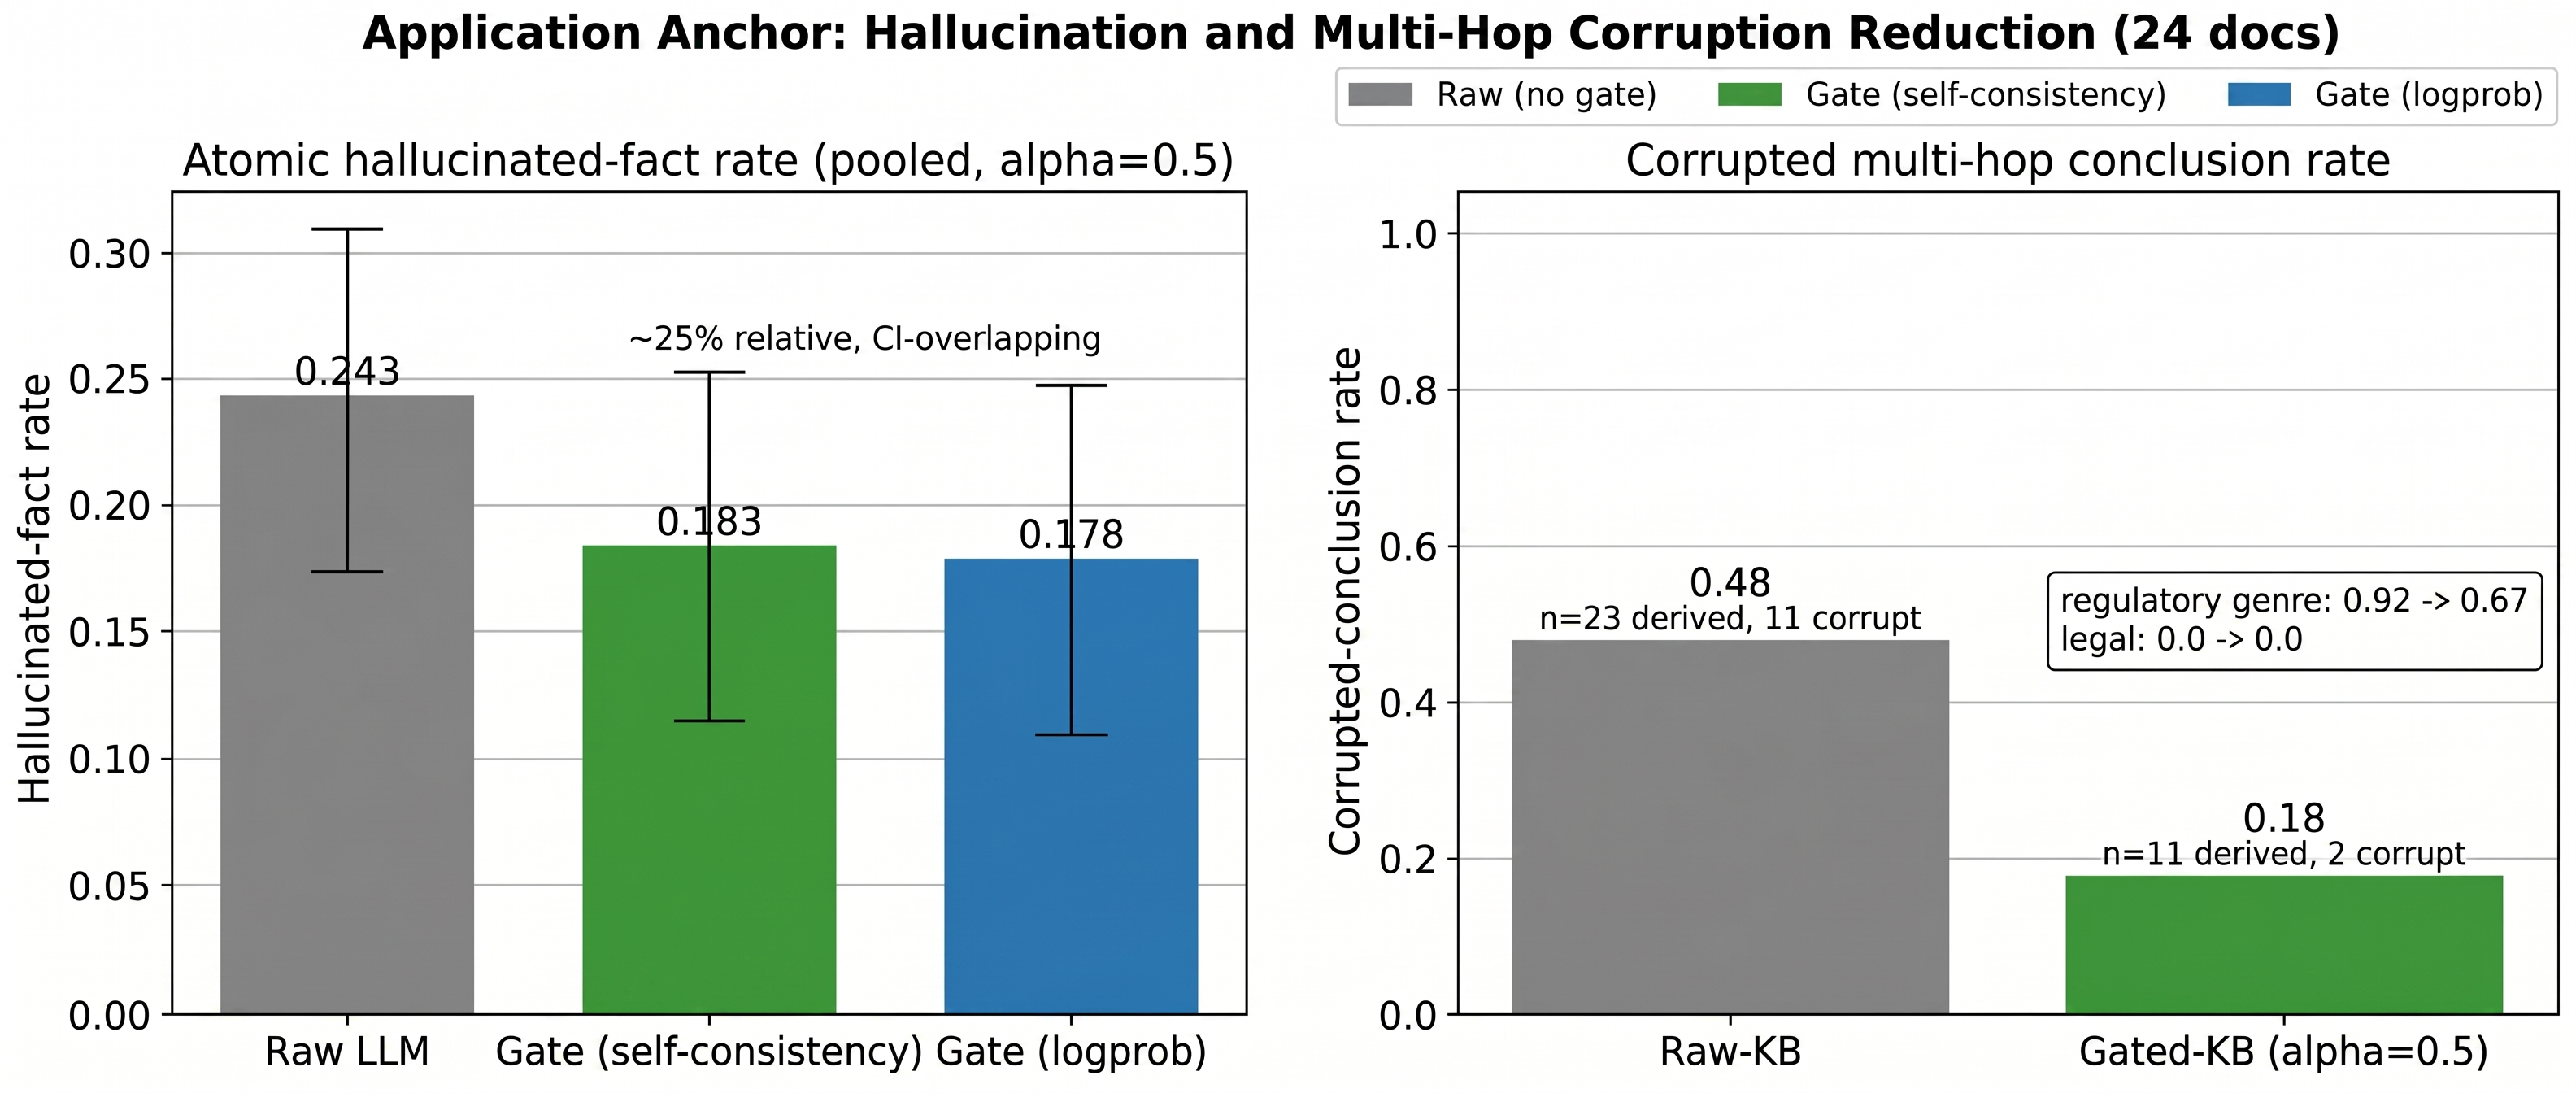
\includegraphics[width=\linewidth,height=0.4\textheight,keepaspectratio]{figures/fig4_v0.jpg}
  \caption{Executed application headline on the 24-document legal/news/regulatory anchor at the certified $\alpha=0.5$. Left: pooled atomic hallucinated-fact rate, raw LLM vs.\ gate---a directional $\sim$25\% reduction (CIs overlap at $n=24$; 0/40 grid cells reach CI separation). Right: corrupted multi-hop conclusion rate drops sharply from raw-KB $0.48$ (23 conclusions) to gated-KB $0.18$ (11 conclusions). The gate's self-report is conservative on this anchor.}
  \label{fig:application}
\end{figure}

\emph{First, the atomic hallucination reduction is directional, not significant.} At the only certified target ($\alpha=0.5$; the $24$-document corpus floors stricter $\alpha$ at zero admissions), the pooled gate hallucinated-fact rate is $0.183$ under self-consistency and $0.178$ under log-probability, versus the $\alpha$-invariant raw-LLM rate of $0.243$---a $\sim 25\%$ relative reduction---but $0$ of $40$ grid cells reach bootstrap-CI separation at $n=24$, so the reduction is directional. The largest single-cell reduction is regulatory under self-consistency: raw $0.439\to$ gate $0.360$. \emph{Second, and in pointed contrast to the CLUTRR multi-hop regime, the gate's self-report here is conservative}---$\widehat{\mathrm{FDR}}\ge$ realized FDR in every one of the $40$ cells---so the second-order disconfirmation does not fire on this anchor. \emph{Third, the multi-hop corruption result is the clearest positive}: the raw-LLM knowledge base derives $23$ conclusions at a $0.48$ corrupted rate, whereas the gated knowledge base at $\alpha=0.5$ derives $11$ conclusions at a $0.18$ corrupted rate, with the regulatory genre dropping from $0.92$ to $0.67$ and legal from---already clean---$0.0$ to $0.0$. Gating removes the premises that would otherwise propagate into corrupted deductions.

\begin{figure}[!htbp]
  \centering
  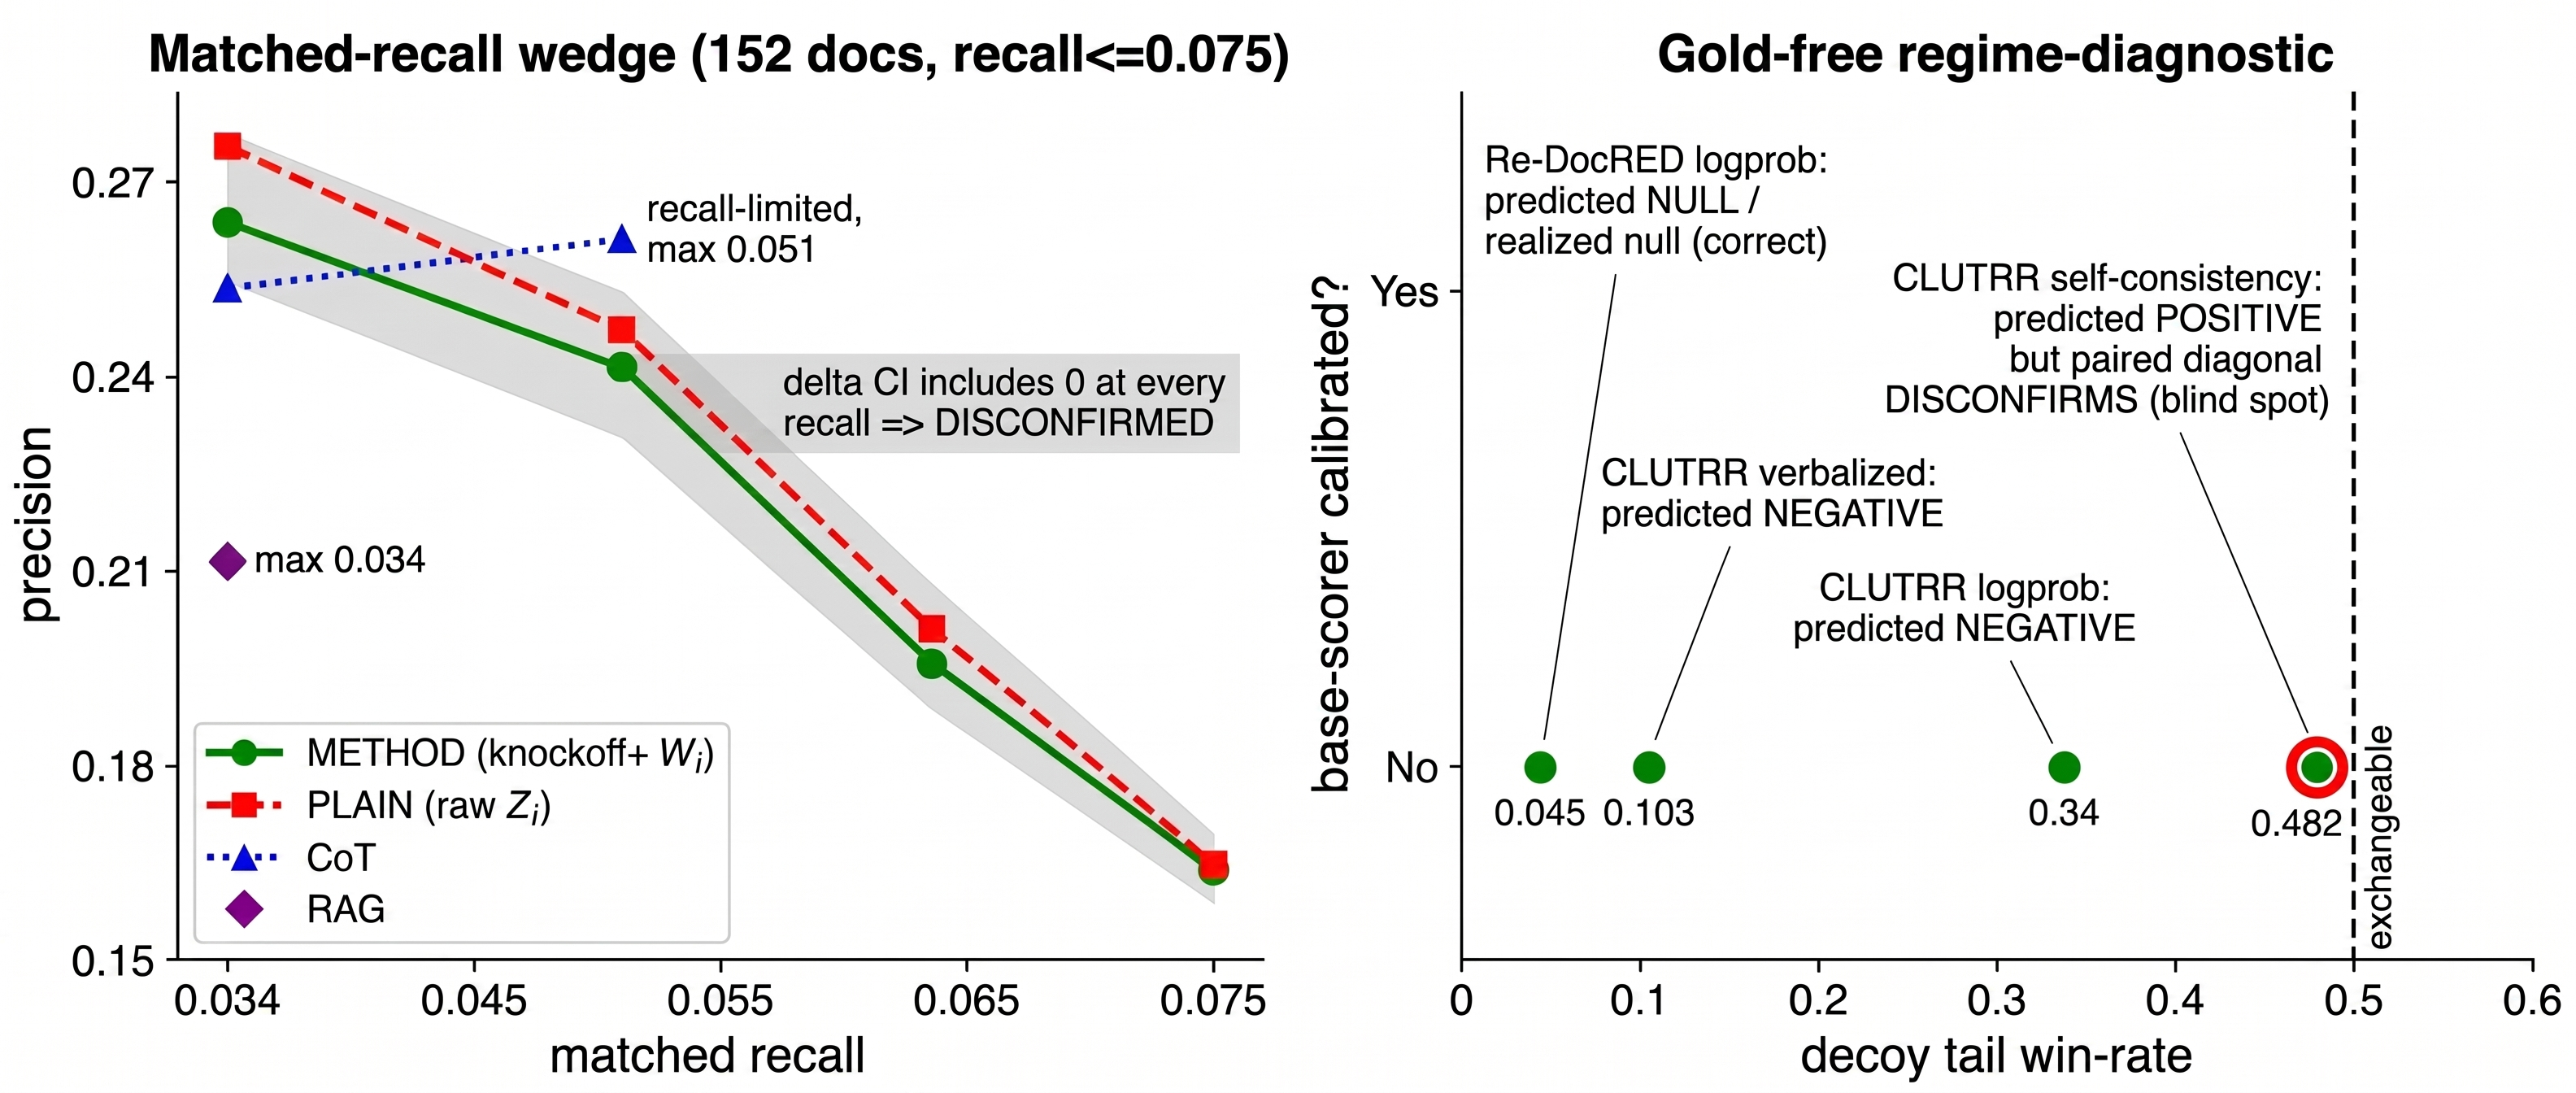
\includegraphics[width=\linewidth,height=0.4\textheight,keepaspectratio]{figures/fig5_v0.jpg}
  \caption{Left: matched-recall precision on 152 Re-DocRED documents (recall ceiling $0.075$). METHOD (knockoff+ $W_i$) and PLAIN (raw $Z_i$) are indistinguishable; CoT and RAG are recall-limited; the wedge is disconfirmed (no point with $\Delta$ CI $>0$). Right: the label-free regime-diagnostic places each anchor/elicitation on (decoy tail win-rate $\times$ base-scorer calibration) and predicts the wedge sign gold-free. Re-DocRED is predicted REDUNDANT (correct). The CLUTRR self-consistency point (win-rate $0.482$) would predict POSITIVE, yet the powered paired diagonal disconfirms it---the marginal diagnostic's blind spot.}
  \label{fig:redocred}
\end{figure}

Every admitted fact enters the symbolic layer with a full certificate, and the pipeline exports auditable trace-graphs (six documents, JSON + Graphviz DOT) whose leaves carry provenance, decoy, and entrapment certificates. For example, the legal proof of \texttt{party\_bound\_effective(Premium Managed Hosting Agreement, AstroNutrition.com, March 1 2005)} resolves through \texttt{has\_party} ($W_i=0.842$, $T=0.129$, $\alpha=0.5$) and \texttt{effective\_date} ($W_i=0.790$), each annotated with the entrapment certificate $(\widehat{\mathrm{FDP}}=0.667, r=1)$; a regulatory proof of \texttt{titled\_obligation(Art.\ 7 GDPR, ...)} exposes a \emph{rejected} leaf (\texttt{obligates}, $W_i=-0.333$) directly in the trace, making the gate's decision human-auditable. Honesty requires three caveats we record at the point of claim: extraction quality on these genres is modest (atomic precision/recall: legal $0.28/0.27$, news $0.29/0.18$, regulatory $0.17/0.42$); $117$ of $210$ reals are gold-undecidable, so hallucination is reported by gold-membership with silver bounds; and the cross-family adjudicator was \emph{dropped} because its agreement with the crisp legal gold was poor ($\kappa=0.10<0.4$), partly because the CUAD gold itself has partial recall.

\subsection{Re-DocRED: disconfirmed wedge, reframed as a gold-free regime-diagnostic (S4)}

We report the operational result at its true, now-corrected scope. Scaling from the prior $36$ documents to the full $152$ confirmatory documents, ranking the identical candidate pool by the knockoff+ statistic $W_i$ does \emph{not} beat ranking by raw confidence $Z_i$ at matched recall: across the recall grid (ceiling $0.075$, the shared METHOD/PLAIN maximum) no point shows a precision gain with bootstrap CI entirely above zero, so the pre-registered verdict is an operational disconfirmation---\emph{at recall $\le0.075$ on 152 documents}. Two reviewer-flagged weaknesses are fixed. All five systems now participate: relaxing the matched-recall floor to the lowest positive maximum recall ($0.034$) gives the recall-limited CoT ($0.051$) and RAG ($0.034$) at least one evaluable point, so no all-null baseline is listed as a comparator. And the multi-hop comparison is \emph{powered}: six gold-justified Wikidata inverse rules densify forward-chained conclusions to $267$ per system (far above the pre-registered power target of $100$), giving a hallucinated-conclusion-rate difference of $-0.004$ (CI $[-0.018,0.008]$)---a precisely null effect, not an underpowered one.

The substantive new contribution is to recast this null as a \emph{prediction}. A label-free regime-diagnostic (zero API calls, no gold) reads four cached signals: the tail decoy win-rate ($0.045$, far below $0.5$ $\Rightarrow$ decoys too easy), the spontaneous-error CDF match (decoy mean $0.165$ vs.\ low-self-consistency real mean $0.857$; KS/MW/permutation all reject $\Rightarrow$ too easy), the $W$-versus-$Z$ ranking divergence (fraction of candidates with $W_i=Z_i$ equal to $0.939$, admitted-set Spearman $\rho=0.991$ $\Rightarrow$ the gate keeps and orders the same facts as the plain threshold, so the wedge is \emph{mechanically} null), and base-scorer calibration (AUC $=0.60$). The diagnostic emits ``GATE REDUNDANT, predicted wedge sign null,'' which the realized wedge confirms (prediction correct). Placed beside the CLUTRR regimes, the diagnostic yields a unifying---and honestly caveated---two-axis picture: gate value rises with base-scorer tail-overconfidence but is \emph{conditional} on decoy exchangeability. The one point this two-axis map gets \emph{wrong} is the very point our calibration diagonal corrects: the CLUTRR self-consistency win-rate of $0.482$ would predict ``gate adds value,'' yet the powered paired diagonal disconfirms it (Section 6.1). That contradiction is not a flaw in the reporting---it is the clearest possible statement of this paper's central finding, that a marginal win-rate cannot certify paired validity.

\subsection{Cost and reproducibility}

The entire iteration ran on commodity CPU: the corrected self-consistency diagonal cost \$0.02 (cache-warm), the application headline \$0.31, and the Re-DocRED regime-diagnostic \$1.08, for $\sim$\$1.4 this iteration and $\sim$\$2.6 cumulative against the \$10 cap, with exact per-call metering and a persistent on-disk cache enabling free resumes. All anchors regenerate deterministically under fixed seeds.

\section{Discussion}

\paragraph{What we now know, and where the certificate breaks.} Decoy-gated extraction is the first label-free FDR knob proposed at the fuzzy-unification boundary, and executing it carefully has taught a precise lesson that a working certificate would have hidden. The validity of a knockoff-style gate at the LLM boundary decomposes into two layers: a \emph{marginal} layer (decoy scores distributed like the model's spontaneous errors), achievable by an aggregation elicitation and verifiable label-free; and a \emph{paired} layer (the false real and its decoy equally likely to win at the cutoff), which the knockoff theorems actually require and which we find can fail even when the marginal layer holds. The standard decoy-quality diagnostics imported from genomics and proteomics live entirely in the marginal layer, so they \emph{over-certify} the gate. This is, to our knowledge, the first demonstration that the marginal/paired distinction is operative---and consequential---when knockoffs are transplanted to LLM scoring.

\paragraph{The honest value proposition.} The gate's \emph{operational} value over plain thresholding is concentrated where the base elicitation is tail-overconfident and the decoys are exchangeable, and is null where the base scorer is already calibrated (Re-DocRED). The gate's \emph{certified-FDR} value is, on present evidence, not established on hard multi-hop families: marginal exchangeability is necessary but not sufficient. What survives unambiguously is the \emph{auditable pipeline}---typed extraction, a quantitatively-reported (if directional) hallucination reduction on genre-faithful documents, a measured drop in corrupted multi-hop conclusions ($0.48\to0.18$), and per-leaf certificates---and the \emph{gold-free regime-diagnostic}, which correctly forecasts where the gate is redundant. These are the deliverables the goal requires, and they do not depend on the missing certificate.

\paragraph{Limitations.} First and foremost, the FDR certificate is disconfirmed on the populable CLUTRR multi-hop family under the diagnostic-validated elicitation; we do not claim label-free FDR control there. Second, the self-detecting diagnostic has a structural blind spot: a marginal win-rate cannot certify paired validity, and at our checkpoint the difficulty ladder is underpowered, so the ``tells you when to trust the gate'' claim is downgraded accordingly. Third, the CLUTRR diagonal is computed on a $40$-document checkpoint; a powered re-run is the immediate next step, though the disconfirmation direction (realized $1.0$, CI above $\alpha^{*}$) is unlikely to reverse. Fourth, the application hallucination reduction is directional, not CI-separated, at $n=24$, and its gold is partly silver. Fifth, we descope two named goal requirements with stated rationale: OpenCyc is discontinued, so we substitute an offline WordNet$\to$SUMO typing stack that supplies taxonomic grounding but not Cyc's assertional commonsense KB; and the executed reasoning layer is deterministic backward chaining, with the ProbLog probabilistic upgrade designed and specified but not yet run.

\paragraph{Connection to the target application.} The pipeline ingests short professionally written documents, types their entities against an upper ontology, translates them to first-order logic, executes multi-hop deductions, and emits auditable trace-graphs on commodity hardware---the operational profile the task demands. The decoy gate is a tunable, label-free hallucination-reduction control that raw LLM generation lacks; what this iteration establishes is precisely the boundary of its statistical guarantee, so a practitioner knows it as an operational filter with measured (directional) benefit and auditable provenance, not as a certified-FDR oracle.

\section{Conclusion}

We formulated the text-to-logic admission boundary as a label-free FDR-control problem, introduced decoy-gated extraction, and---taking the reviewers' methodology objection as the organizing question---re-ran the calibration diagonal under the elicitation the win-rate diagnostic actually validates. The corrected diagonal disconfirms the gate's FDR certificate on the error-dense multi-hop family (realized FDR $1.0$ at $\alpha^{*}=0.5$, CI $[0.66,1.0]$), and we localize the cause: self-consistency restores \emph{marginal} decoy exchangeability (decoy$\approx$spontaneous-error, KS $p=0.058$; $\neq$ true-positive, KS $p=5\times10^{-9}$) but not the \emph{paired} sign-flip property knockoff+ requires, so a marginal diagnostic over-certifies the gate. Where the goal lives, the pipeline nonetheless delivers: on $24$ genre-faithful documents it cuts the corrupted multi-hop conclusion rate from $0.48$ to $0.18$ and the atomic hallucination rate $\sim 25\%$ (directional) with conservative self-report and exported auditable trace-graphs; on $152$ Re-DocRED documents the operational wedge is disconfirmed at recall $\le0.075$ and a gold-free regime-diagnostic predicts that null correctly. Future work, in priority order, is to (1) build a \emph{paired}-exchangeability diagnostic and decoy family that close the marginal-paired gap rather than measuring around it; (2) execute the powered self-consistency diagonal and the ProbLog probabilistic upgrade; (3) develop the regime-diagnostic into a deployment-time gate-applicability test; and (4) tighten the conservative $+1$ floor where validity permits.

\bibliographystyle{plainnat}
\bibliography{references}

\end{document}
